% Koko
\documentclass[blue,normal,cn]{elegantnote}
\usepackage{array}
\usepackage{courier}
\usepackage{xcolor}
\definecolor{light-gray}{gray}{0.95}
\newcommand{\code}[1]{\colorbox{light-gray}{\texttt{#1}}}
\newfontfamily\courier{Courier New}
\lstset{linewidth=1.1\textwidth,
	numbers=left,
	basicstyle=\small\courier,
	numberstyle=\tiny\courier,
	keywordstyle=\color{blue}\courier,
	commentstyle=\it\color[cmyk]{1,0,1,0}\courier, 
	stringstyle=\it\color[RGB]{128,0,0}\courier,
	frame=single,
	backgroundcolor=\color[RGB]{245,245,244},
	breaklines,
	extendedchars=false, 
	xleftmargin=2em,xrightmargin=2em, aboveskip=1em,
	tabsize=4, 
	showspaces=false
	basicstyle=\small\courier
}
\title{操作系统基本课程实验报告}
\version{$\aleph$}
\date{\today}

\begin{document}
\author{
\begin{tabular}[t]{c@{\extracolsep{4em}}c} 
    于海鑫  & 范乾一 \\
    2017211240 & 2017211219
\end{tabular}
}
\maketitle

\tableofcontents

\section{实验环境}
我们进行实验的主要有两套环境,两套环境的配置如下:
\begin{itemize}
  \item Windows 10 1903 配合其内置的 WSL 环境
  \item Kubuntu 19.10
\end{itemize}

在实验报告的运行结果内,可以由 \texttt{bash} 的 \texttt{prompt} 
进行分辨。显示 \texttt{name1e5s@DESKTOP-D8BIQ3U} 的为 WSL 环境
,显示 \texttt{name1e5s@asgard} 的则是 Kubuntu。

这两套环境的硬件配置相同,都是 Intel I7-7700HQ 与 16GB DDR3 内存,
我们实验报告内部的分析都是根据这两套软硬件配置进行的。

\section{系统安装实验}
\subsection{实验目的}
从网络上下载的 ISO 中安装任一 Linux 发行版,例如 Ubuntu 19.10,
建立后续实验的运行环境。
\subsection{实验内容}
\subsubsection{安装虚拟机}
\begin{enumerate}
  \item 打开北邮人 BT,搜索 VMware Workstation Pro,获取
  \href{https://bt.byr.cn/details.php?id=284764&hit=1}{下载链接}
  \item 打开程序进行安装
  \begin{figure}[!htbp]
    \centering
    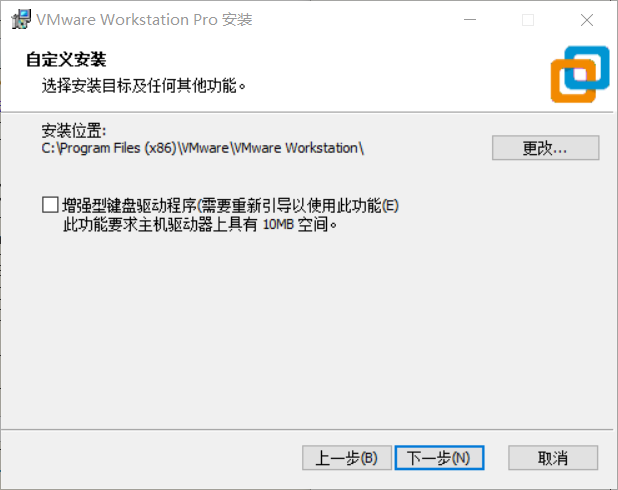
\includegraphics[width=.8\textwidth]{fig/lab-1/fig1-1}
    \caption{VMware Workstation Pro 15 安装界面}
    \label{fig:VMwareInstall}
  \end{figure}
  \item 一路下一步进行程序的安装
  \item 在安装的最后,选择许可证,输入神秘代码 \code{CG392-4PX5J-H816Z-HYZNG-PQRG2}
  \item 双击桌面上的 ``VMware Workstation Pro'' 图标,看到如图~\ref{fig:VMwareMain}~
  所示界面,表示虚拟机安装成功
  \begin{figure}[!htbp]
    \centering
    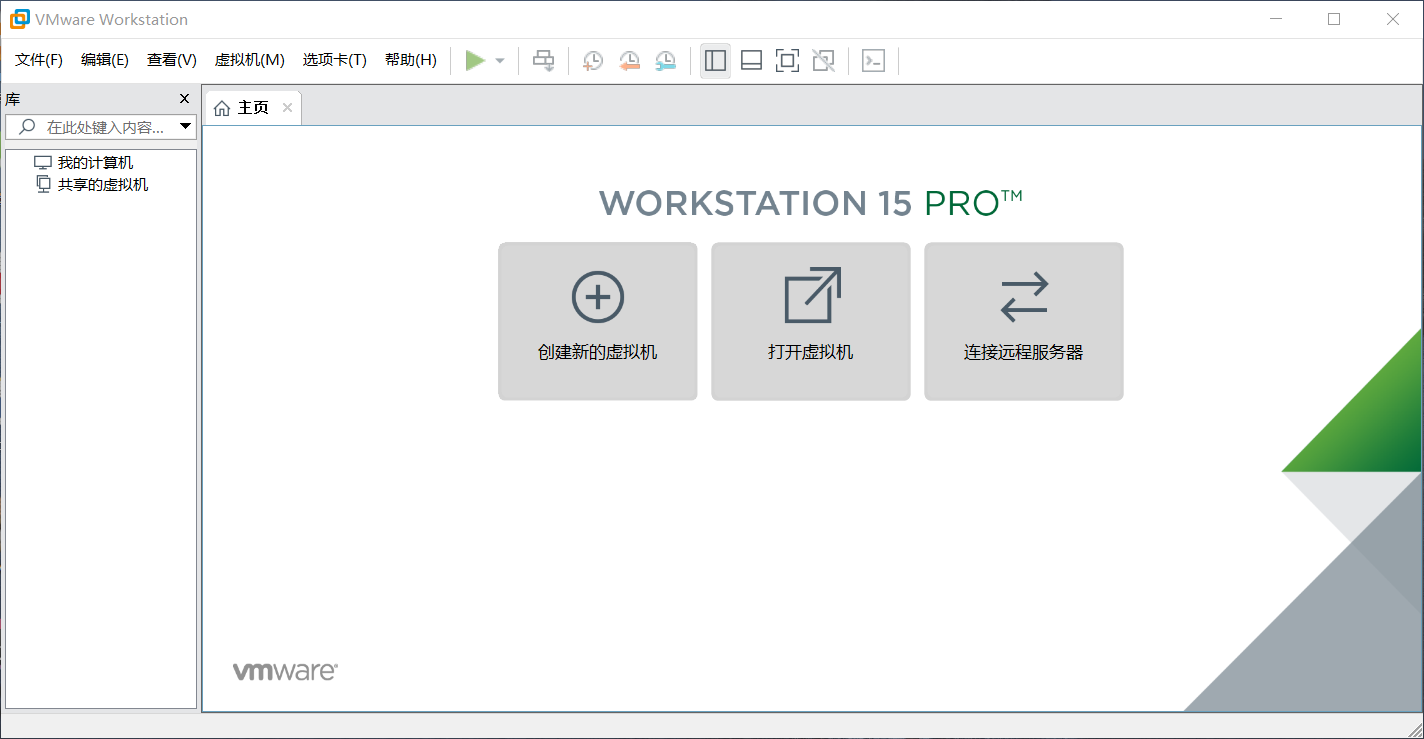
\includegraphics[width=.8\textwidth]{fig/lab-1/fig1-2}
    \caption{VMware Workstation Pro 15 安装界面}
    \label{fig:VMwareMain}
  \end{figure}
\end{enumerate}
\subsubsection{安装 Ubuntu 19.10}
\begin{enumerate}
  \item 首先登陆 \href{https://mirrors.tuna.tsinghua.edu.cn/}{清华大学开源软件镜像站}
  获取 Ubuntu 19.10 的镜像
  \item 打开 VMware Workstation Pro 15,选择创建虚拟机,按照我们的需求确定对应的虚拟机配置,
  因为 VMware Workstation Pro 对于 Ubuntu 等常见的 Linux 发行版提供了
  ``简易安装''的选项,我们只需等待虚拟机自动为我们安装。需要注意的是,在
  Ubuntu 的安装过程中如果联网可能会导致 Ubuntu 尝试进行更新,
  该过程通常会很慢,因此建议在安装过程中关闭互联网的连接。
  \begin{figure}[!htbp]
    \centering
    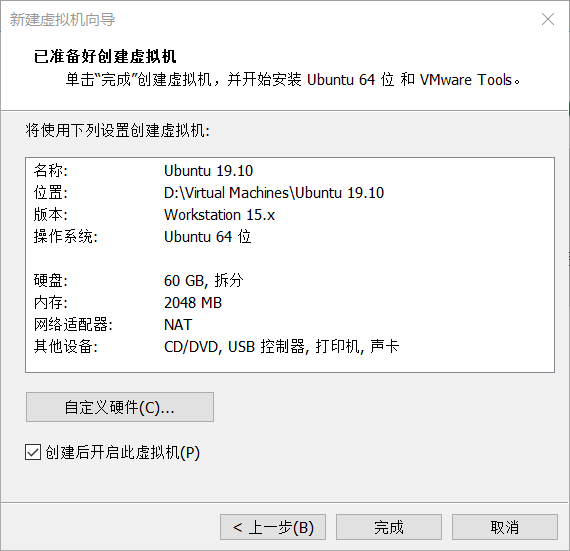
\includegraphics[width=.8\textwidth]{fig/lab-1/fig2-1}
    \caption{最终配置的结果}
    \label{fig:ConfFinal}
  \end{figure}
  \begin{figure}[!htbp]
    \centering
    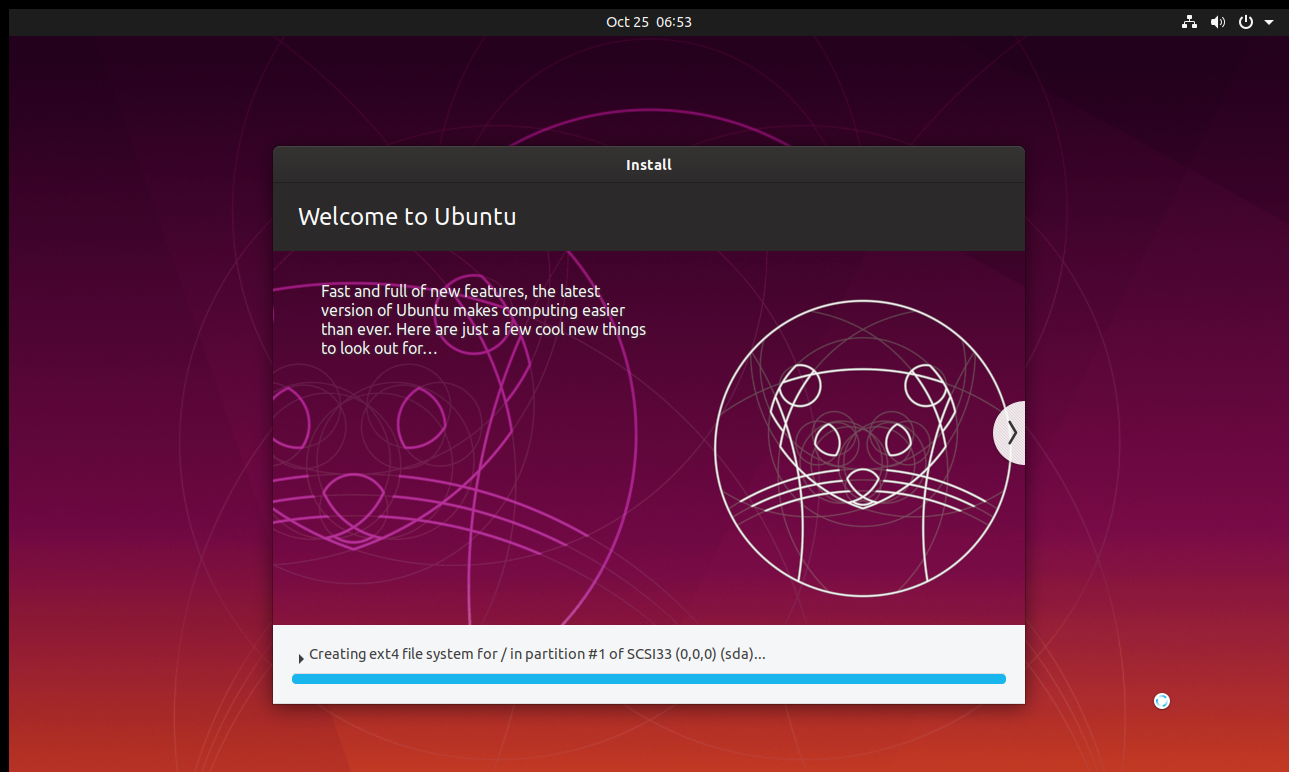
\includegraphics[width=.8\textwidth]{fig/lab-1/fig2-2}
    \caption{Ubuntu 安装界面}
    \label{fig:UbuntuInstall}
  \end{figure}
  \item Ubuntu 会在安装后的第一次重启安装 \code{open-vm-tools} 
  以支持一些方便使用的功能,因此第一次开机会比较慢
  \begin{figure}[!htbp]
    \centering
    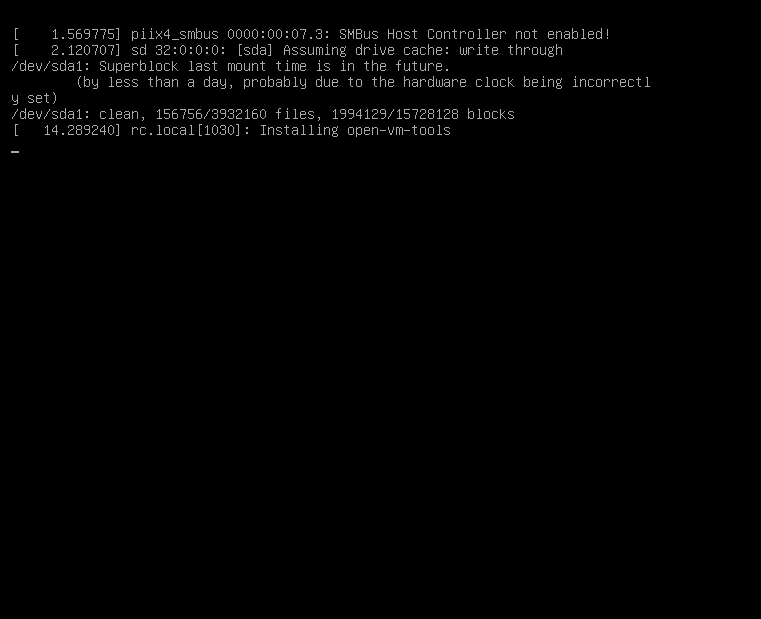
\includegraphics[width=.8\textwidth]{fig/lab-1/fig2-3}
    \caption{open-vm-tools 安装界面}
    \label{fig:open-vm-tools}
  \end{figure}
  \item 在一些初始化工作结束后,我们就可以看到 Ubuntu 的登陆界面,
  可以注意到这一版本的登陆界面的背景色相比之前的版本比较浅
  \begin{figure}[!htbp]
    \centering
    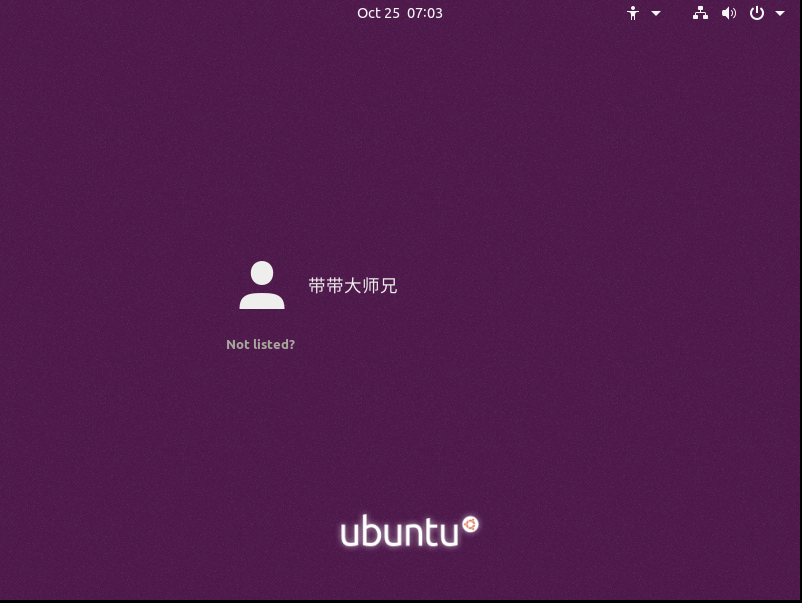
\includegraphics[width=.8\textwidth]{fig/lab-1/fig2-4}
    \caption{Ubuntu 19.10 登陆界面}
    \label{fig:UbuntuLogin}
  \end{figure}
  \item 选择之前创建的账户并输入密码,即可进入 Ubuntu 桌面
  \begin{figure}[!htbp]
    \centering
    
\includegraphics[width=.8\textwidth]{fig/lab-1/fig2-5}
    \caption{Ubuntu 19.10 主界面}
    \label{fig:UbuntuMain}
  \end{figure}
\end{enumerate}

\subsubsection{配置环境}
\begin{enumerate}
  \item \textbf{修改源为清华源}\ 按下 \code{Ctrl + Alt + T} 
  打开 Terminal,输入 \\
  \code{sudo sed -i 's/us.archive.ubuntu.com/mirrors.tuna.tsinghua.edu.cn/g'} \\
  \code{/etc/apt/sources.list}
  修改软件源为清华源,之后通过 \\
  \code{sudo apt update \&\& sudo apt upgrade} 同步软件库并进行
  更新
  \item \textbf{准备 Linux 内核的编译环境}\ 在终端内输入 \\
  \code{sudo apt build-dep linux linux-image-\$(uname -r)}
  获取所需的软件包,按照 \href{https://wiki.ubuntu.com/Kernel/BuildYourOwnKernel#Build_Environment}{Ubuntu Wiki}
  所述,我们还需要执行 \code{sudo apt install} \\
  \code{libncurses-dev flex bison openssl libssl-dev dkms} \\
  \code{libelf-dev libudev-dev libpci-dev libiberty-dev autoconf}
  以安装编译内核所需的依赖
  \item \textbf{获取内核的源码}\ 使用 \\
  \code{apt source linux-image-\$(uname -r)} 
  即可获取我们后续需要修改的 Linux 源码
  \item \textbf{安装广受好评的代码 VS Code}
  \begin{lstlisting}
wget https://go.microsoft.com/fwlink/?LinkID=760868 -O /tmp/code.deb
sudo apt install /tmp/code.deb
  \end{lstlisting}
\end{enumerate}

\section{Linux 内核实验}
\subsection{观察 Linux 行为}
\subsubsection{实验目的}
学习 Linux 内核、进程、存储和其他资源的一些重要特性。
通过使用 \code{/proc} 文件系统接口, 编写一个程序
检查反映机器平衡负载、进程资源利用率方面的各种内核值, 
学会使用 \code{/proc} 文件系统这种内核状态检查机制。
\subsubsection{实验内容}
编写一个默认版本的程序通过检查内核状态报告 Linux 内核行为。
程序应该在标准输出上打印以下值:
\begin{itemize}
  \item CPU类型和型号
  \item 所使用的 Linux 内核版本
  \item 从系统最后一次启动以来已经经历了多长时间(天,小时和分钟)
  \item 总共有多少CPU时间执行在用户态,系统态,空闲态
  \item 配置内存数量,当前可用内存数,磁盘读写请求数
  \item 内核上下文转换数
  \item 系统启动到目前创建了多少进程
\end{itemize}

\subsubsection{程序源代码清单}

\begin{lstlisting}[language=C]
#include <stdio.h>
#include <sys/time.h>
#include <time.h>

void print_info(const char *file_path, const char *format) {
    char line_buf[1024];                // 1K should be enough
    FILE *fp = fopen(file_path, "r");   // Open file
    fgets(line_buf, 1024, fp);          // Read file into line buffer
    printf(format, line_buf);           // Print file
    fclose(fp);                         // Close file
}

void print_info_long(const char *file_path, const char *prompt) {
    char line_buf[1024];                // 1K should be enough
    FILE *fp = fopen(file_path, "r");   // Open file
    printf("===== BEGIN %s =====\n", prompt);
    while(fgets(line_buf, 1024, fp)) {
        printf("%s", line_buf);
    }
    printf("====== END %s ======\n", prompt);
    fclose(fp);                         // Close file
}


void print_time(void) {
    struct timeval tv;
    struct tm* ptm;
    char time_string[40];
    long milliseconds;

    gettimeofday (&tv, NULL); // Get current time from GLIBC
    ptm = localtime (&tv.tv_sec); // Convert time to local time
    strftime (time_string, sizeof (time_string), "%Y-%m-%d %H:%M:%S", ptm); // Convert time to human-readable string
    printf(" ::: REPORT AT %s ::: \n", time_string);
}

int main(int argc, char *argv) {
    print_time();
    // 输出机器的 hostname
    print_info("/proc/sys/kernel/hostname", "Machine Hostname: %s");
    // 输出机器的内核版本
    print_info("/proc/version", "Kernel Version: %s");
    // 输出开机时长
    print_info("/proc/uptime", "Total Uptime: %s");
    // 输出 CPU 的详细信息
    print_info_long("/proc/cpuinfo", "CPU INFO");
    // 获取并输出内核的信息
    print_info_long("/proc/meminfo", "MEM INFO");
    // 输出开机以来的统计信息,格式如下:
    // name,user,nice,system,idle,iowait,irrq,softirq,steal,guest,guest_nice
    // 详见 https://supportcenter.checkpoint.com/supportcenter/portal?eventSubmit_doGoviewsolutiondetails=&solutionid=sk65143
    print_info_long("/proc/stat", "CURRENT STATUS");
    // 输出操作系统最近的负载信息
    // The first three fields in this file are load average figures giving the 
    // number of jobs in the run queue (state R) or waiting for disk I/O (state 
    // D) averaged over 1, 5, and 15 minutes. They are the same as the load 
    // average numbers given by uptime(1) and other programs. The fourth field 
    // consists of two numbers separated by a slash (/). The first of these is 
    // the number of currently runnable kernel scheduling entities (processes, 
    // threads). The value after the slash is the number of kernel scheduling 
    // entities that currently exist on the system. The fifth field is the PID of 
    // the process that was most recently created on the system.
    print_info("/proc/loadavg", "Load Average: %s");
    return 0;
}
\end{lstlisting}
\subsubsection{运行结果}
\begin{lstlisting}
name1e5s@asgard:~/lab2$ gcc 2.1.c
name1e5s@asgard:~/lab2$ ./a.out
 ::: REPORT AT 2019-10-26 21:40:43 :::
Machine Hostname: asgard
Kernel Version: Linux version 5.3.0-18-generic (buildd@lcy01-amd64-027) (gcc version 9.2.1 20190909 (Ubuntu 9.2.1-8ubuntu1)) #19-Ubuntu SMP Tue Oct 8 20:14:06 UTC 2019
Total Uptime: 7452.57 28872.35
===== BEGIN CPU INFO =====
processor       : 0
vendor_id       : GenuineIntel
cpu family      : 6
model           : 158
model name      : Intel(R) Core(TM) i7-7700HQ CPU @ 2.80GHz
stepping        : 9
microcode       : 0xb4
cpu MHz         : 2808.004
cache size      : 6144 KB
physical id     : 0
siblings        : 2
core id         : 0
cpu cores       : 2
apicid          : 0
initial apicid  : 0
fpu             : yes
fpu_exception   : yes
cpuid level     : 22
wp              : yes
flags           : fpu vme de pse tsc msr pae mce cx8 apic sep mtrr pge mca cmov pat pse36 clflush mmx fxsr sse sse2 ss ht syscall nx pdpe1gb rdtscp lm constant_tsc arch_perfmon nopl xtopology tsc_reliable nonstop_tsc cpuid pni pclmulqdq ssse3 fma cx16 pcid sse4_1 sse4_2 x2apic movbe popcnt tsc_deadline_timer aes xsave avx f16c rdrand hypervisor lahf_lm abm 3dnowprefetch cpuid_fault invpcid_single pti ssbd ibrs ibpb stibp fsgsbase tsc_adjust bmi1 avx2 smep bmi2 invpcid mpx rdseed adx smap clflushopt xsaveopt xsavec xsaves arat md_clear flush_l1d arch_capabilities
bugs            : cpu_meltdown spectre_v1 spectre_v2 spec_store_bypass l1tf mds swapgs
bogomips        : 5616.00
clflush size    : 64
cache_alignment : 64
address sizes   : 43 bits physical, 48 bits virtual
power management:

processor       : 1
vendor_id       : GenuineIntel
cpu family      : 6
model           : 158
model name      : Intel(R) Core(TM) i7-7700HQ CPU @ 2.80GHz
stepping        : 9
microcode       : 0xb4
cpu MHz         : 2808.004
cache size      : 6144 KB
physical id     : 0
siblings        : 2
core id         : 1
cpu cores       : 2
apicid          : 1
initial apicid  : 1
fpu             : yes
fpu_exception   : yes
cpuid level     : 22
wp              : yes
flags           : fpu vme de pse tsc msr pae mce cx8 apic sep mtrr pge mca cmov pat pse36 clflush mmx fxsr sse sse2 ss ht syscall nx pdpe1gb rdtscp lm constant_tsc arch_perfmon nopl xtopology tsc_reliable nonstop_tsc cpuid pni pclmulqdq ssse3 fma cx16 pcid sse4_1 sse4_2 x2apic movbe popcnt tsc_deadline_timer aes xsave avx f16c rdrand hypervisor lahf_lm abm 3dnowprefetch cpuid_fault invpcid_single pti ssbd ibrs ibpb stibp fsgsbase tsc_adjust bmi1 avx2 smep bmi2 invpcid mpx rdseed adx smap clflushopt xsaveopt xsavec xsaves arat md_clear flush_l1d arch_capabilities
bugs            : cpu_meltdown spectre_v1 spectre_v2 spec_store_bypass l1tf mds swapgs
bogomips        : 5616.00
clflush size    : 64
cache_alignment : 64
address sizes   : 43 bits physical, 48 bits virtual
power management:

processor       : 2
vendor_id       : GenuineIntel
cpu family      : 6
model           : 158
model name      : Intel(R) Core(TM) i7-7700HQ CPU @ 2.80GHz
stepping        : 9
microcode       : 0xb4
cpu MHz         : 2808.004
cache size      : 6144 KB
physical id     : 1
siblings        : 2
core id         : 0
cpu cores       : 2
apicid          : 2
initial apicid  : 2
fpu             : yes
fpu_exception   : yes
cpuid level     : 22
wp              : yes
flags           : fpu vme de pse tsc msr pae mce cx8 apic sep mtrr pge mca cmov pat pse36 clflush mmx fxsr sse sse2 ss ht syscall nx pdpe1gb rdtscp lm constant_tsc arch_perfmon nopl xtopology tsc_reliable nonstop_tsc cpuid pni pclmulqdq ssse3 fma cx16 pcid sse4_1 sse4_2 x2apic movbe popcnt tsc_deadline_timer aes xsave avx f16c rdrand hypervisor lahf_lm abm 3dnowprefetch cpuid_fault invpcid_single pti ssbd ibrs ibpb stibp fsgsbase tsc_adjust bmi1 avx2 smep bmi2 invpcid mpx rdseed adx smap clflushopt xsaveopt xsavec xsaves arat md_clear flush_l1d arch_capabilities
bugs            : cpu_meltdown spectre_v1 spectre_v2 spec_store_bypass l1tf mds swapgs
bogomips        : 5616.00
clflush size    : 64
cache_alignment : 64
address sizes   : 43 bits physical, 48 bits virtual
power management:

processor       : 3
vendor_id       : GenuineIntel
cpu family      : 6
model           : 158
model name      : Intel(R) Core(TM) i7-7700HQ CPU @ 2.80GHz
stepping        : 9
microcode       : 0xb4
cpu MHz         : 2808.004
cache size      : 6144 KB
physical id     : 1
siblings        : 2
core id         : 1
cpu cores       : 2
apicid          : 3
initial apicid  : 3
fpu             : yes
fpu_exception   : yes
cpuid level     : 22
wp              : yes
flags           : fpu vme de pse tsc msr pae mce cx8 apic sep mtrr pge mca cmov pat pse36 clflush mmx fxsr sse sse2 ss ht syscall nx pdpe1gb rdtscp lm constant_tsc arch_perfmon nopl xtopology tsc_reliable nonstop_tsc cpuid pni pclmulqdq ssse3 fma cx16 pcid sse4_1 sse4_2 x2apic movbe popcnt tsc_deadline_timer aes xsave avx f16c rdrand hypervisor lahf_lm abm 3dnowprefetch cpuid_fault invpcid_single pti ssbd ibrs ibpb stibp fsgsbase tsc_adjust bmi1 avx2 smep bmi2 invpcid mpx rdseed adx smap clflushopt xsaveopt xsavec xsaves arat md_clear flush_l1d arch_capabilities
bugs            : cpu_meltdown spectre_v1 spectre_v2 spec_store_bypass l1tf mds swapgs
bogomips        : 5616.00
clflush size    : 64
cache_alignment : 64
address sizes   : 43 bits physical, 48 bits virtual
power management:

====== END CPU INFO ======
===== BEGIN MEM INFO =====
MemTotal:        8026040 kB
MemFree:         1738604 kB
MemAvailable:    6201220 kB
Buffers:           80480 kB
Cached:          4323088 kB
SwapCached:          112 kB
Active:          2633716 kB
Inactive:        2771088 kB
Active(anon):     867116 kB
Inactive(anon):   128896 kB
Active(file):    1766600 kB
Inactive(file):  2642192 kB
Unevictable:          16 kB
Mlocked:              16 kB
SwapTotal:       2097148 kB
SwapFree:        2095856 kB
Dirty:               188 kB
Writeback:             0 kB
AnonPages:       1001228 kB
Mapped:           359508 kB
Shmem:              7668 kB
KReclaimable:     359100 kB
Slab:             513240 kB
SReclaimable:     359100 kB
SUnreclaim:       154140 kB
KernelStack:       13056 kB
PageTables:        19232 kB
NFS_Unstable:          0 kB
Bounce:                0 kB
WritebackTmp:          0 kB
CommitLimit:     6110168 kB
Committed_AS:    5113800 kB
VmallocTotal:   34359738367 kB
VmallocUsed:       48484 kB
VmallocChunk:          0 kB
Percpu:           107008 kB
HardwareCorrupted:     0 kB
AnonHugePages:         0 kB
ShmemHugePages:        0 kB
ShmemPmdMapped:        0 kB
CmaTotal:              0 kB
CmaFree:               0 kB
HugePages_Total:       0
HugePages_Free:        0
HugePages_Rsvd:        0
HugePages_Surp:        0
Hugepagesize:       2048 kB
Hugetlb:               0 kB
DirectMap4k:      405312 kB
DirectMap2M:     6836224 kB
DirectMap1G:     1048576 kB
====== END MEM INFO ======
===== BEGIN CURRENT STATUS =====
cpu  30608 4116 34965 2875047 11766 0 3746 0 0 0
cpu0 8639 1202 8974 718437 2056 0 944 0 0 0
cpu1 7225 966 8611 721501 1854 0 500 0 0 0
cpu2 8018 971 9034 718111 2962 0 1106 0 0 0
cpu3 6725 976 8344 716997 4891 0 1195 0 0 0
ctxt 4387813
btime 1572143790
processes 38700
procs_running 2
procs_blocked 0
softirq 2173065 3 597872 1516 303852 153212 0 3641 540495 0 572474
====== END CURRENT STATUS ======
Load Average: 0.04 0.01 0.09 2/689 38573
\end{lstlisting}
\subsection{内核定时器}
\subsubsection{实验目的}
学习掌握内核定时器的实现原理和方法,
建立一种用户空间机制来测量多线程程序的执行时间。
\subsubsection{ITIMER 介绍}

间隔定时器(Interval Timer,简称 ITIMER)是一种
使用间隔值作为计时方式的定时器。在定时器启动后,其间隔
值不断地减小,当间隔值减小到  0 的时候,我们就将之视为
到期。在 Linux 内核内,为每个 task 都提供了三个间隔定时器:

\begin{itemize}
  \item \textbf{ITIMER\_REAL}\ 在启动该计时器后,无论进程是否在运行,
  内核都会在每个时钟滴答将其间隔计数器减 1,当减到 0 时,
  内核向进程发送 \code{SIGALRM} 信号。  
  \item \textbf{ITIMER\_VIRTUAL}\ 只有在进程在用户态执行时
  该计时器内的计数器才会自减,当减到 0 时,内核向进程发送 \textbf{SIGVTALRM}
  信号。
  \item \textbf{ITIMER\_PROF}\ 只有在进程在执行时(用户态与内核态均可)该计时器内的计数器才会自减,
  当减到 0 时,内核向进程发送 \code{SIGPROF} 信号。
\end{itemize}

\subsubsection{用定时器 \textbf{ITIMER\_REAL} 实现\code{gettimeofday}
的功能。使其一秒钟产生一个信号,计算已经过的秒数}

代码如下:
\begin{lstlisting}[language=C]
#include <stdio.h>
#include <signal.h>

#include <sys/time.h>

static void sighandle(int);

static int second = 0;

static void sighandle(int sig) {
    second ++;
    printf("%d\n", second);
}

int main(void) {
    // Set SIGALRM handler
    signal(SIGALRM, sighandle);

    // Fill the fucking struct
    struct itimerval timerval;
	timerval.it_interval.tv_sec = 1;
	timerval.it_interval.tv_usec = 0;
	timerval.it_value.tv_sec = 1;
	timerval.it_value.tv_usec = 0;
    setitimer(ITIMER_REAL, &timerval, NULL);
    
    // Geadloop
    while(1);
}
\end{lstlisting}

运行结果如下:
\begin{lstlisting}
name1e5s@ubuntu:~/lab2$ gcc 2.2.1.c
name1e5s@ubuntu:~/lab2$ ./a.out
1
2
3
4
5
6
7
8
9
10
11
12
13
14
15
^C
name1e5s@ubuntu:~/lab2$
\end{lstlisting}

\subsubsection{记录一个进程运行时所占用的
\textbf{real time, cpu time,user time ,kernel time}}
代码如下:

\begin{lstlisting}[language=C]
#include <sys/time.h>
#include <stdio.h>
#include <signal.h>

static void sighandle(int);

static long realsecond = 0;
static long vtsecond = 0;
static long profsecond = 0;

static void sighandle(int sig) {
    switch(sig) {
        case SIGALRM:
            realsecond += 10;
            break;
        case SIGVTALRM:
            vtsecond += 10;
            break;
        case SIGPROF:
            profsecond += 10;
            break;
        default:
            break;
    }
}

int fib(int n) {
    if(n == 0 || n == 1) {
        return 1;
    }

    return fib(n - 1) + fib(n - 2);
}

void print_time(const struct itimerval *tv, long second, const char *prompt) {
    long sec_count = 10 - tv->it_value.tv_sec;
	long msec_count = (1000000 - tv->it_value.tv_usec)/1000;
	printf("%s = %ld sec, %ld msec\n", prompt, second + sec_count,msec_count);
}

int main(void) {
    static struct itimerval realt,virtt,proft;

    // Set signal handler
    signal(SIGALRM, sighandle);
    signal(SIGVTALRM, sighandle);
    signal(SIGPROF, sighandle);

    // Fill the fucking struct
    struct itimerval timerval;
	timerval.it_interval.tv_sec = 10;
	timerval.it_interval.tv_usec = 0;
	timerval.it_value.tv_sec = 10;
	timerval.it_value.tv_usec = 0;

    // Set the fucking timer
    setitimer(ITIMER_REAL, &timerval, NULL);
	setitimer(ITIMER_VIRTUAL,&timerval,NULL);
	setitimer(ITIMER_PROF,&timerval,NULL);

    // Waste time...
    fib(22);
    for (int i = 0; i < 20000; i++) {
        puts("I Can Eat Glass and It Won't Hurt Me");
    }

    // Get the timer
	getitimer(ITIMER_PROF,&proft);
	getitimer(ITIMER_REAL,&realt);
	getitimer(ITIMER_VIRTUAL,&virtt);

    // Print time
    print_time(&realt, realsecond, "Real Time");
    print_time(&proft, profsecond, "CPU Time");
    print_time(&virtt, vtsecond, "User Time");

    // Calculate Kernel Time and Print
    long t1 = (10 - proft.it_value.tv_sec)*1000 + (1000000 - proft.it_value.tv_usec)/1000 + profsecond*10000;
	long t2 = (10 - virtt.it_value.tv_sec)*1000 + (1000000 - virtt.it_value.tv_usec)/1000 + vtsecond*10000;
	long moresec = (t1 - t2)/1000;
	long moremsec = (t1 - t2) % 1000;
	printf("Kernel Time = %ld sec, %ld msec\n", moresec, moremsec);

    return 0;
}
\end{lstlisting}

运行结果如下:

\begin{lstlisting}
name1e5s@ubuntu:~/lab2$ gcc 2.2.2.c
name1e5s@ubuntu:~/lab2$ ./a.out | tail
I Can Eat Glass and It Won't Hurt Me
I Can Eat Glass and It Won't Hurt Me
I Can Eat Glass and It Won't Hurt Me
I Can Eat Glass and It Won't Hurt Me
I Can Eat Glass and It Won't Hurt Me
I Can Eat Glass and It Won't Hurt Me
Real Time = 1 sec, 45 msec
CPU Time = 1 sec, 40 msec
User Time = 0 sec, 1000 msec
Kernel Time = 0 sec, 40 msec
name1e5s@ubuntu:~/lab2$
\end{lstlisting}

\subsubsection{编写一个主程序产生两个子进程,分别递归计算N =20,30,36的 Fibonacci 序列。分别对三个进程计算相应的 real time, cpu time,user time ,kernel time}

代码如下:

\begin{lstlisting}[language=C]
#include <sys/time.h>
#include <sys/wait.h>
#include <stdio.h>
#include <signal.h>
#include <unistd.h>

void sighandle(int);

long realsecond = 0;
long vtsecond = 0;
long profsecond = 0;

void sighandle(int sig) {
    switch(sig) {
        case SIGALRM:
            realsecond += 10;
            break;
        case SIGVTALRM:
            vtsecond += 10;
            break;
        case SIGPROF:
            profsecond += 10;
            break;
        default:
            break;
    }
}

int fib(int n) {
    if(n == 0 || n == 1) {
        return 1;
    }

    return fib(n - 1) + fib(n - 2);
}

void print_time(const struct itimerval *tv, long second, const char *prompt, int n) {
    long sec_count = 10 - tv->it_value.tv_sec;
	long msec_count = (1000000 - tv->it_value.tv_usec)/1000;
	printf(prompt, n, second + sec_count, msec_count);
}

int fib_forked(int n) {
    struct itimerval realt,virtt,proft;

    // Set signal handler
    signal(SIGALRM, sighandle);
    signal(SIGVTALRM, sighandle);
    signal(SIGPROF, sighandle);

    // Fill the fucking struct
    struct itimerval timerval;
	timerval.it_interval.tv_sec = 10;
	timerval.it_interval.tv_usec = 0;
	timerval.it_value.tv_sec = 10;
	timerval.it_value.tv_usec = 0;

    // Set the fucking timer
    setitimer(ITIMER_REAL, &timerval, NULL);
	setitimer(ITIMER_VIRTUAL,&timerval,NULL);
	setitimer(ITIMER_PROF,&timerval,NULL);

    // Waste time...
    // Print info
    printf("fib(%d) = %d \n", n, fib(n));

    // Get the timer
	getitimer(ITIMER_PROF,&proft);
	getitimer(ITIMER_REAL,&realt);
	getitimer(ITIMER_VIRTUAL,&virtt);

    // Print time
    print_time(&realt, realsecond, "Fib(%d) Real Time = %ld sec, %ld msec\n", n);
    print_time(&proft, profsecond, "Fib(%d) CPU Time = %ld sec, %ld msec\n", n);
    print_time(&virtt, vtsecond, "Fib(%d) User Time = %ld sec, %ld msec\n", n);

    // Calculate Kernel Time and Print
    long t1 = (10 - proft.it_value.tv_sec)*1000 + (1000000 - proft.it_value.tv_usec)/1000 + profsecond*10000;
	long t2 = (10 - virtt.it_value.tv_sec)*1000 + (1000000 - virtt.it_value.tv_usec)/1000 + vtsecond*10000;
	long moresec = (t1 - t2)/1000;
	long moremsec = (t1 - t2) % 1000;
	printf("Kernel Time = %ld sec, %ld msec\n", moresec, moremsec);

    return 0;
}

int main(void) {
    int pid_fib10 = fork();
    if(pid_fib10 == 0) {
        fib_forked(10);
    } else {
        int pid_fib20 = fork();
        if(pid_fib20 == 0) {
            fib_forked(20);
        } else {
            int pid_fib36 = fork();
            if(pid_fib36 == 0) {
                fib_forked(36);
            }
        }
    }
    wait(NULL);
    wait(NULL);
    wait(NULL);
    return 0;
}
\end{lstlisting}

输出结果如下:

\begin{lstlisting}
name1e5s@ubuntu:~/lab2$ gcc 2.2.3.c
name1e5s@ubuntu:~/lab2$ ./a.out
fib(10) = 89
Fib(10) Real Time = 1 sec, 0 msec
Fib(10) CPU Time = 0 sec, 996 msec
Fib(10) User Time = 0 sec, 996 msec
Kernel Time = 0 sec, 0 msec
fib(20) = 10946
Fib(20) Real Time = 1 sec, 0 msec
Fib(20) CPU Time = 0 sec, 996 msec
Fib(20) User Time = 0 sec, 996 msec
Kernel Time = 0 sec, 0 msec
fib(36) = 24157817
Fib(36) Real Time = 1 sec, 109 msec
Fib(36) CPU Time = 1 sec, 104 msec
Fib(36) User Time = 1 sec, 104 msec
Kernel Time = 0 sec, 0 msec
\end{lstlisting}

\subsection{内核模块}
\subsubsection{实验目的}
模块是 Linux 系统的一种特有机制,可用以动态扩展操作系统
内核功能。编写实现某些特定功能的模块,将其作为内核的一部分
在管态下运行。本实验通过内核模块编程在 \code{/porc} 文件系统中实现
系统时钟的读操作接口。
\subsubsection{实验内容}
设计并构建一个在 \code{/proc} 文件系统中的内核模块 \code{clock},
支持 \code{read()} 操作,\code{read()} 返回值为一字符串,
其中包块一个空各分开的两个子串,为别代表 \code{xtime.tv\_sec} 
和 \code{xtime.tv\_usec}
\subsubsection{实验原理}
Linux 模块是一些可以作为独立程序来编译的函数和数据类型的集合。
在装载这些模块式,将它的代码链接到内核中。Linux 模块可以在内核
启动时装载,也可以在内核运行的过程中装载。如果在模块装载之前就调
用了动态模块的一个函数,那么这次调用将会失败。如果这个模块已被加
载,那么内核就可以使用系统调用,并将其传递到模块中的相应函数。
\subsubsection{实验过程}
\paragraph{编写内核模块}
我们要实现的内核模块主要包括标记为 \code{\_\_init} 的初始化函数
以及标记为 \code{\_\_exit} 的退出函数,还有描述文件相关的 
\code{file\_operations} 结构体以及用以处理读取/写入的相关函数。
因为 \code{do\_gettimeofday} 函数在 \code{5.0} 
以上的内核上被删除了,我们需要使用如下代码来模拟该函数的行为:
\begin{lstlisting}[language=C]
void do_gettimeofday(struct timeval *tv) {
	struct timespec now;

	getnstimeofday(&now);
	tv->tv_sec = now.tv_sec;
	tv->tv_usec = now.tv_nsec/1000;
}
\end{lstlisting}
全部代码如下:
\begin{lstlisting}[language=C]
#include <linux/init.h>
#include <linux/module.h>
#include <linux/kernel.h>
#include <linux/proc_fs.h>
#include <linux/seq_file.h>
#include <linux/time.h>
 
MODULE_LICENSE("GPL");
MODULE_AUTHOR("name1e5s");
MODULE_DESCRIPTION("A harmless clock.");
MODULE_VERSION("0.1");

static const char *file_name = "clock";

// Removed in kernel 5.0, use getnstimeofday instead.
// F**K IT
void do_gettimeofday(struct timeval *tv) {
	struct timespec now;

	getnstimeofday(&now);
	tv->tv_sec = now.tv_sec;
	tv->tv_usec = now.tv_nsec/1000;
}

static int fill_info(struct seq_file *m, void *v) {
    struct timeval xtime;
    do_gettimeofday(&xtime);
    seq_printf(m, "%ld %ld\n", xtime.tv_sec, xtime.tv_usec);
	return 0;
}

static int open(struct inode *inode, struct file *file) {
	return single_open(file, fill_info, NULL);
}

static const struct file_operations fops = {
	.llseek = seq_lseek,
	.open = open,
	.owner = THIS_MODULE,
	.read = seq_read,
	.release = single_release,
};

static int __init clock_init(void) {
    printk(KERN_INFO "Clock: Hello from the harmless clock!\n");
    proc_create(file_name, 0, NULL, &fops);
    return 0;
}


static void __exit clock_exit(void){
    printk(KERN_INFO "Clock: Goodbye from the harmless clock!\n");
    remove_proc_entry(file_name, NULL);
}

module_init(clock_init);
module_exit(clock_exit);
\end{lstlisting}

\paragraph{编写 Makefile} 为了让我们的代码能在 Linux 内核源码树上编译
为模块文件,我们需要编写如下 Makefile
\begin{lstlisting}
obj-m+=clock.o

all:
	make -C /lib/modules/$(shell uname -r)/build/ M=$(PWD) modules
clean:
	make -C /lib/modules/$(shell uname -r)/build/ M=$(PWD) clean
\end{lstlisting}

\paragraph{编译运行}
\begin{lstlisting}
name1e5s@ubuntu:~/lab2/2.3$ make
make -C /lib/modules/5.3.0-18-generic/build/ M=/home/name1e5s/lab2/2.3 modules
make[1]: Entering directory '/usr/src/linux-headers-5.3.0-18-generic'
  CC [M]  /home/name1e5s/lab2/2.3/clock.o
  Building modules, stage 2.
  MODPOST 1 modules
  CC      /home/name1e5s/lab2/2.3/clock.mod.o
  LD [M]  /home/name1e5s/lab2/2.3/clock.ko
make[1]: Leaving directory '/usr/src/linux-headers-5.3.0-18-generic'
name1e5s@ubuntu:~/lab2/2.3$ modinfo ./clock.ko
filename:       /home/name1e5s/lab2/2.3/./clock.ko
version:        0.1
description:    A harmless clock.
author:         name1e5s
license:        GPL
srcversion:     BE5E6FC2EF7FFD62690068C
depends:
retpoline:      Y
name:           clock
vermagic:       5.3.0-18-generic SMP mod_unload
name1e5s@ubuntu:~/lab2/2.3$ sudo insmod clock.ko
name1e5s@ubuntu:~/lab2/2.3$ cat /proc/clock
1572161313 290301
name1e5s@ubuntu:~/lab2/2.3$ sudo rmmod clock.ko
name1e5s@ubuntu:~/lab2/2.3$ cat /var/log/kern.log
Oct 27 00:28:23 ubuntu kernel: [17512.252405] Clock: Hello from the harmless clock!
Oct 27 00:28:39 ubuntu kernel: [17528.682741] Clock: Goodbye from the harmless clock!
\end{lstlisting}
我们已经看到了内核模块注册和退出时的信息,现在我们使用指导书提供的测试样例进行测试。


\paragraph{测试}
我们使用如下代码进行测试:
\begin{lstlisting}[language=C]
#include <stdio.h>
#include <sys/time.h>
#include <fcntl.h>

int main(void) {
	struct timeval getSystemTime;
	char procClockTime[256];
	int infile,len;

	gettimeofday(&getSystemTime,NULL);

	infile = open("/proc/clock",O_RDONLY);
	len = read(infile,procClockTime,256);
	close(infile);

	procClockTime[len] = '\0';

    printf("SystemTime is %d %d\nProcClockTime is %s\n",
        getSystemTime.tv_sec,
        getSystemTime.tv_usec,
        procClockTime);

	sleep(1);
    return 0;
} 
\end{lstlisting}
测试的输出如下:
\begin{lstlisting}
name1e5s@ubuntu:~/lab2/2.3$ gcc 2.3.c
2.3.c: In function ‘main’:
2.3.c:13:8: warning: implicit declaration of function ‘read’; did you mean ‘fread’? [-Wimplicit-function-declaratio ]
   13 |  len = read(infile,procClockTime,256);
      |        ^~~~
      |        fread
2.3.c:14:2: warning: implicit declaration of function ‘close’; did you mean ‘pclose’? [-Wimplicit-function-declaration]
   14 |  close(infile);
      |  ^~~~~
      |  pclose
2.3.c:18:28: warning: format ‘%d’ expects argument of type ‘int’, but argument 2 has type ‘__time_t’ {aka ‘long int’} [-Wformat=]
   18 |     printf("SystemTime is %d %d\nProcClockTime is %s\n",
      |                           ~^
      |                            |
      |                            int
      |                           %ld
   19 |         getSystemTime.tv_sec,
      |         ~~~~~~~~~~~~~~~~~~~~
      |                      |
      |                      __time_t {aka long int}
2.3.c:18:31: warning: format ‘%d’ expects argument of type ‘int’, but argument 3 has type ‘__suseconds_t’ {aka ‘long int’} [-Wformat=]
   18 |     printf("SystemTime is %d %d\nProcClockTime is %s\n",
      |                              ~^
      |                               |
      |                               int
      |                              %ld
   19 |         getSystemTime.tv_sec,
   20 |         getSystemTime.tv_usec,
      |         ~~~~~~~~~~~~~~~~~~~~~
      |                      |
      |                      __suseconds_t {aka long int}
2.3.c:23:2: warning: implicit declaration of function ‘sleep’ [-Wimplicit-function-declaration]
   23 |  sleep(1);
      |  ^~~~~
name1e5s@ubuntu:~/lab2/2.3$ ./a.out
SystemTime is 1572161601 335857
ProcClockTime is 1572161601 335870
\end{lstlisting}
忽略由于给的示例代码不规范造成的 Warning 外,
可以看出通过我们实现的模块获取的时间和使用 
\code{gettimeofday} 函数获取的时间相差无几。

\subsection{系统调用}
\subsubsection{实验目的}
向现有Linux内核加入一个新的系统调用从而在内核空间中实现对用户空间的读写。
例如,设计并实现一个新的内核函数 \code{mycall()},
此函数通过一个引用参数的调用返回当前系统时间,功能上基本与
\code{gettimeofday()} 相同。
\subsubsection{关于 Linux 更新导致的代码变更}
\begin{itemize}
  \item CVE-2009-0029 以后,Linux 开始使用 \code{SYSCALL\_DEFINEx}
  系列的宏以确保传参的安全
  \item \code{do\_gettimeofday} 已死,我们使用 \code{getnstimeofday}
  模拟其行为
  \item \code{sys\_call\_table[]} 现在使用可读性更强的
  \code{.tbl}
  文件实现,其位置为 \\
  \code{arch/x86/entry/syscall/syscall\_64.tbl}
  \item \code{\_syscall1} 宏已被弃用,我们使用 \code{syscall} 函数来
  调用我们自己添加的系统调用
\end{itemize}
\subsubsection{实验内容}
\paragraph{添加新调用}
\begin{enumerate}
  \item 在 \code{kernel/sys.c} 内添加如下代码
  \begin{lstlisting}[language=C]
void do_gettimeofday(struct timeval *tv) {
  struct timespec now;
  getnstimeofday(&now);
  tv->tv_sec = now.tv_sec;
  tv->tv_usec = now.tv_nsec/1000;
}
   
int do_mysyscall(struct timeval *tv) {
  struct timeval kernel_tv;
  do_gettimeofday(&kernel_tv);
  return copy_to_user(tv, &kernel_tv, sizeof(kernel_tv));
}
   
SYSCALL_DEFINE1(mysyscall, struct timeval *, tv) {
return do_mysyscall(tv);
}
  \end{lstlisting}
  \item 在 \code{arch/x86/entry/syscall/syscall\_64.tbl} 
  里面添加如下代码
  \begin{lstlisting}
    436	common	mysyscall			__x64_sys_mysyscall
  \end{lstlisting}
\end{enumerate}

\paragraph{编译内核}
在这里,我们使用 Debian 系提供的 \code{make-kpkg} 工具编译内核
\begin{lstlisting}
fakeroot make-kpkg --initrd --append-to-version=-lab \
kernel-image kernel-headers -j8
\end{lstlisting}
在等待了大约一个半小时后,编译结束,

\paragraph{测试}
在安装生成的内核 \code{.deb} 文件并重启切换到新的内核后,使用
如下代码进行测试:
\begin{lstlisting}[language=C]
#define _GNU_SOURCE
#include <unistd.h>
#include <sys/syscall.h>
#include <sys/types.h>
int main(int argc, char *argv[]) {
  struct timeval gettime;
  struct timeval mycalltime;
   
  gettimeofday(&gettime,NULL);
  syscall(436, &mycalltime);
  printf("gettimeofday:%d%d\n",gettime.tv_sec,gettime.tv_usec);
  printf("mycall:%d%d\n",mycalltime.tv_sec,mycalltime.tv_usec);
}
\end{lstlisting}

测试结果如下:
\begin{lstlisting}
name1e5s@ubuntu:~/lab2$ gcc 2.4.c 
name1e5s@ubuntu:~/lab2$ ./a.out 
gettimeofday:1572172804385006
mycall:1572172804385008
\end{lstlisting}
结果符合预期。

\section{进程管理实验 —— Shell 编程}
\subsection{实验目的}
通过编写shell程序,了解子进程的创建
和父进程与子进程间的协同,获得多进程程序的编程经验。
\subsection{实验内容}
编写一个带有重定向和管道功能的 shell 程序。
\subsection{实现思路}
通过 \code{fork} 创建子进程,用 \code{execvp} 
更改子进程代码,用 \code{wait} 等待子进程结束。
这三个系统调用可以很好地创建多进程。

对于 pipe 操作,我们通过使用 \code{dup*} 系列系统调用来替换
进程的文件描述符来实现。

输入解析为编译原理课程内容,在此不再介绍。

\subsubsection{实现代码}
\begin{lstlisting}[language=C]
#include <stdio.h>
#include <stdlib.h>
#include <stdbool.h>
#include <string.h>

#include <unistd.h>
#include <sys/types.h>
#include <sys/stat.h>
#include <fcntl.h>

#define MAXARGLEN 64
#define MAXARGS 128
#define BUFFER_SIZE 1024

#define TOK_END 0
#define TOK_STR 1
#define TOK_APP 2
#define TOK_OUT 3
#define TOK_INF 4
#define TOK_PIP 5

#define TYPE_IN 1
#define TYPE_OUT 2
#define TYPE_APPEND 3
#define TYPE_INOUT 4
#define TYPE_INAPPEND 5

static char command_buffer[BUFFER_SIZE];
static char token_buffer[BUFFER_SIZE];
static int command_index;

typedef enum {
    TYPE_EXEC,
    TYPE_PIPE,
    TYPE_REDI,
    TYPE_EROR
} type_t;

typedef struct meta_command {
    type_t type;
} meta_command;

typedef struct exec_command {
    type_t type;
    int argc;
    char *argv[MAXARGS];
} exec_command;

typedef struct redi_command {
    type_t type;
    exec_command *real_command;
    char in_file[MAXARGLEN];
    char out_file[MAXARGLEN];
    int redi_type;
} redi_command;

typedef struct pipe_command {
    type_t type;
    meta_command *left;
    meta_command *right;
} pipe_command;

void get_command() {
    command_index = 0;
	for(int i = 0; i < 1024; i++)
		command_buffer[i] = 0;
    printf("=> ");
    gets(command_buffer);
}

bool is_valid_char(char c) {
    if(c == '>' || c == '<' || c == '|' || c == '\t' || c == '\n' || c == ' ')
        return false;
    return true;
}

int get_basic_string() {
    int token_index = 0;
    while(command_buffer[command_index] != '\0' &&
            is_valid_char(command_buffer[command_index])) {
        token_buffer[token_index++] = command_buffer[command_index];
        command_index ++;
    }
    token_buffer[token_index++] = '\0';
    return token_index - 1 == 0 ? TOK_END : TOK_STR;
}

int lex() {
    int token_index = 0;
    token_buffer[0] = '\0';
    while(command_buffer[command_index] != '\0') {
        switch (command_buffer[command_index]) {
            case ' ':
            case '\n':
            case '\t':
            case '\r':
                command_index += 1;
                break;
            case '>':
                if(command_buffer[command_index + 1] == '>') {
                    token_buffer[0] = '>';
                    token_buffer[1] = '>';
                    token_buffer[2] = '\0';
                    command_index += 2;
                    return TOK_APP;
                } else {
                    token_buffer[0] = '>';
                    token_buffer[1] = '\0';
                    command_index += 1;
                    return TOK_OUT;
                }
            case '<':
                token_buffer[0] = '<';
                token_buffer[1] = '\0';
                command_index += 1;
                return TOK_INF;
            case '|':
                token_buffer[0] = '|';
                token_buffer[1] = '\0';
                command_index += 1;
                return TOK_PIP;
            default:
                return get_basic_string();
        }
    }
    return TOK_END;
}

char peek() {
    int i = 0;
    while(command_buffer[command_index + i] != '\0' && (command_buffer[command_index + i] == ' ' || command_buffer[command_index + i] == '\t'))
        i ++;
    return command_buffer[command_index + i];
}

pipe_command *build_pipe_command(meta_command *left, meta_command *right) {
    pipe_command *command = malloc(sizeof(pipe_command));
    memset(command, 0, sizeof(pipe_command));
    command->type = TYPE_PIPE;
    command->left = left;
    command->right = right;
    return command;
}

redi_command *build_redi_command(exec_command *real_command, char *in_file, char *out_file, int redi_type) {
    redi_command *command = malloc(sizeof(redi_command));
    memset(command, 0, sizeof(redi_command));
    command->type = TYPE_REDI;
    command->real_command = real_command;
    strcpy(command->in_file, in_file);
    strcpy(command->out_file, out_file);
    command->redi_type = redi_type;
    return command;
}

meta_command *parse_command() {
    exec_command *command = malloc(sizeof(exec_command));
    memset(command, 0, sizeof(exec_command));
    command->type = TYPE_EXEC;
    int token_type;
    while ((token_type = lex()) == TOK_STR) {
        command->argv[command->argc] = malloc(strlen(token_buffer) + 1);
        strcpy(command->argv[command->argc], token_buffer);
        command->argc ++;
    }
    switch (token_type) {
        case TOK_PIP:
            return (meta_command *)build_pipe_command((meta_command *)command,  (meta_command *)parse_command());
        case TOK_INF:
        case TOK_OUT:
        case TOK_APP:
            lex();
            int curr_type = token_type;
            char buffered_op[MAXARGLEN];
            strcpy(buffered_op, token_buffer);
            int next_type = lex();
            if(next_type == TOK_STR) {
                command->type = TYPE_EROR;
                return (meta_command *)command;
            } else if(next_type == TOK_PIP) {
                if(curr_type == TOK_INF)
                    return (meta_command *)build_pipe_command((meta_command *) build_redi_command(
                            command, buffered_op, "", TYPE_IN), (meta_command *)parse_command());
                if(curr_type == TOK_OUT)
                    return (meta_command *)build_pipe_command((meta_command *) build_redi_command(
                            command, "", buffered_op, TYPE_OUT), (meta_command *)parse_command());
                if(curr_type == TOK_APP)
                    return (meta_command *)build_pipe_command((meta_command *) build_redi_command(
                            command, "", buffered_op, TYPE_APPEND), (meta_command *)parse_command());
            } else if(next_type == TOK_END) {
                if(curr_type == TOK_INF)
                    return (meta_command *) build_redi_command(command, buffered_op, "", TYPE_IN);
                if(curr_type == TOK_OUT)
                    return (meta_command *) build_redi_command(command, "", buffered_op, TYPE_OUT);
                if(curr_type == TOK_APP)
                    return (meta_command *) build_redi_command(command, "", buffered_op, TYPE_APPEND);
            } else if (next_type == TOK_OUT || next_type == TOK_APP) {
                if(curr_type == TOK_OUT || curr_type == TOK_APP || lex() != TOK_STR) {
                    command->type = TYPE_EROR;
                    return (meta_command *)command;
                } else {
                    return (meta_command *) build_redi_command(command, token_buffer,
                            buffered_op, next_type == TOK_OUT ? TYPE_INOUT : TYPE_INAPPEND);
                }
            } else if(next_type == TOK_INF) {
                if(curr_type == TOK_INF || lex() != TOK_STR) {
                    command->type = TYPE_EROR;
                    return (meta_command *)command;
                } else {
                    return (meta_command *) build_redi_command(command, buffered_op, token_buffer, curr_type == TOK_OUT ? TYPE_INOUT : TYPE_INAPPEND);
                }
            }
            break;
        default:
            return (meta_command *)command;
    }
}

void run_command(meta_command *command) {
    int fd;
    int pipe_fd[2];
    switch (command->type) {
    case TYPE_EXEC:
        execvp(((exec_command *)command)->argv[0], ((exec_command *)command)->argv);
        break;
    case TYPE_REDI:
        switch(((redi_command *)command)->redi_type) {
        case TYPE_IN:
            if((fd = open(((redi_command *)command)->in_file, O_RDONLY)) == -1) {
                puts("Open file failed.");
                return;
            }
            dup2(fd, STDIN_FILENO);
            close(fd);
            break;
        case TYPE_APPEND:
            if((fd = open(((redi_command *)command)->out_file, O_WRONLY | O_APPEND | O_CREAT, 0666)) == -1) {
                puts("Open file failed.");
                return;
            }
            dup2(fd, STDOUT_FILENO);
            close(fd);
            break;
        case TYPE_OUT:
            if((fd = open(((redi_command *)command)->out_file, O_WRONLY | O_CREAT, 0666)) == -1) {
                puts("Open file failed.");
                return;
            }
            dup2(fd, STDOUT_FILENO);
            close(fd);
            break;
        case TYPE_INOUT:
            if((fd = open(((redi_command *)command)->out_file, O_WRONLY | O_CREAT, 0666)) == -1) {
                puts("Open file failed.");
                return;
            }
            dup2(fd, STDOUT_FILENO);
            close(fd);
            if((fd = open(((redi_command *)command)->in_file, O_RDONLY)) == -1) {
                puts("Open file failed.");
                return;
            }
            dup2(fd, STDIN_FILENO);
            close(fd);
            break;
        case TYPE_INAPPEND:
            if((fd = open(((redi_command *)command)->out_file, O_WRONLY | O_APPEND | O_CREAT, 0666)) == -1) {
                puts("Open file failed.");
                return;
            }
            dup2(fd, STDOUT_FILENO);
            close(fd);
            if((fd = open(((redi_command *)command)->in_file, O_RDONLY)) == -1) {
                puts("Open file failed.");
                return;
            }
            dup2(fd, STDIN_FILENO);
            close(fd);
            break;
        }
        run_command((meta_command *)((redi_command *)command)->real_command);
        break;
    case TYPE_PIPE:
        pipe(pipe_fd);
        if(fork() == 0) {
            dup2(pipe_fd[1], STDOUT_FILENO);
            close(pipe_fd[0]);
            close(pipe_fd[1]);
            run_command((meta_command *)((pipe_command *)command)->left);
        }
        if(fork() == 0) {
            dup2(pipe_fd[0], STDIN_FILENO);
            close(pipe_fd[0]);
            close(pipe_fd[1]);
            run_command((meta_command *)((pipe_command *)command)->left);
        }
        wait();
        wait();
        break;
    default:
        break;
    }
}

int main() {
    while(1) {
        get_command();
		puts(command_buffer);
        if (strncmp(command_buffer, "exit", 4) == 0) {
            exit(0);
        }
        if(fork() == 0) {
            meta_command *command = parse_command();
            run_command(command);
        }
        wait();
    }
    return 0;
}
\end{lstlisting}
\subsection{运行结果}
\begin{lstlisting}
name1e5s@ubuntu:~$ gcc Lab-3.c
Lab-3.c: In function ‘get_command’:
Lab-3.c:66:5: warning: implicit declaration of function ‘gets’; did you mean ‘fgets’? [-Wimplicit-function-declaration]
   66 |     gets(command_buffer);
      |     ^~~~
      |     fgets
Lab-3.c: In function ‘run_command’:
Lab-3.c:295:9: warning: implicit declaration of function ‘wait’ [-Wimplicit-function-declaration]
  295 |         wait();
      |         ^~~~
/usr/bin/ld: /tmp/ccjpGWCM.o: in function `get_command':
Lab-3.c:(.text+0x30): warning: the `gets' function is dangerous and should not be used.
name1e5s@ubuntu:~$ ./a.out
=> ls -la > test.txt
=> cat test.txt
total 136
drwxr-xr-x 20 name1e5s name1e5s  4096 Oct 28 07:34 .
drwxr-xr-x  3 root     root      4096 Oct 25 06:56 ..
-rwxrwxr-x  1 name1e5s name1e5s 17840 Oct 28 07:34 a.out
-rw-------  1 name1e5s name1e5s  3068 Oct 28 07:29 .bash_history
-rw-r--r--  1 name1e5s name1e5s   220 Oct 25 06:56 .bash_logout
-rw-r--r--  1 name1e5s name1e5s  3771 Oct 25 06:56 .bashrc
drwxr-x--- 15 name1e5s name1e5s  4096 Oct 28 07:23 .cache
drwxr-x--- 15 name1e5s name1e5s  4096 Oct 27 03:35 .config
drwxr-xr-x  2 name1e5s name1e5s  4096 Oct 25 07:05 Desktop
drwxr-xr-x  2 name1e5s name1e5s  4096 Oct 25 07:05 Documents
drwxr-xr-x  2 name1e5s name1e5s  4096 Oct 25 07:05 Downloads
drwxr-xr-x  2 name1e5s name1e5s  4096 Oct 25 07:23 .fontconfig
drwx------  3 name1e5s name1e5s  4096 Oct 25 07:04 .gnupg
drwxr-xr-x  3 name1e5s name1e5s  4096 Oct 27 03:40 lab2
-rwxrw-rw-  1 name1e5s name1e5s 10486 Oct 28 07:29 Lab-3.c
drwx------  3 name1e5s name1e5s  4096 Oct 25 07:05 .local
drwxr-xr-x  2 name1e5s name1e5s  4096 Oct 25 07:05 Music
drwxr-xr-x  2 name1e5s name1e5s  4096 Oct 25 07:05 Pictures
drwx------  3 name1e5s name1e5s  4096 Oct 25 07:42 .pki
-rw-r--r--  1 name1e5s name1e5s   807 Oct 25 06:56 .profile
drwxr-xr-x  2 name1e5s name1e5s  4096 Oct 25 07:05 Public
drwx------  2 name1e5s name1e5s  4096 Oct 25 08:15 .ssh
-rw-r--r--  1 name1e5s name1e5s     0 Oct 25 07:12 .sudo_as_admin_successful
drwxr-xr-x  2 name1e5s name1e5s  4096 Oct 25 07:05 Templates
-rw-rw-r--  1 name1e5s name1e5s  1744 Oct 28 07:33 test.txt
drwxr-xr-x  2 name1e5s name1e5s  4096 Oct 25 07:05 Videos
drwxr-xr-x  3 name1e5s name1e5s  4096 Oct 25 07:42 .vscode
drwxrwxr-x  5 name1e5s name1e5s  4096 Oct 25 08:17 .vscode-server
-rw-r--r--  1 name1e5s name1e5s   280 Oct 25 08:17 .wget-hsts
=> exit
name1e5s@ubuntu:~$
\end{lstlisting}

\section{存储管理实验 —— 虚拟存储器管理}
\subsection{实验目的}
学习Linux虚拟存储实现机制;编写代码,
测试虚拟存储系统的缺页错误(缺页中断)发生频率。
\subsection{实验内容}
修改存储管理软件以便可以判断特定进程或者整个系统产生的缺页情况,达到一下目标
\begin{itemize}
  \item 预置缺页频率参数
  \item 报告当前缺页频率
\end{itemize}
\subsection{实验原理}
由于每发生一次缺页都要进入缺页中断服务函数 \code{do\_page\_fault}
一次,所以可以认为执行函数的次数就是系统发生缺页的次数。因
此可以定义一个全局的变量 \code{pfcount} 作为计数变量,
在执行 \code{do\_page\_fault} 时,该变量加 1。
系统经历的时间可以利用原有系统的变量 \code{jiffies},
这是一个系统计时器。在内核加载以后开始计时,以10ms为计时单位。
之后我们通过 \code{/proc} 文件系统以模块的方式提供内核
变量的访问接口。在 \code{/proc} 文件系统下建立文件 \code{pfcount} 和 \code{jiffies}。

\subsection{实验代码}
我们对 Linux 的修改如下:
\begin{lstlisting}
From bce00e670e18b025e7c0a347e24d23a7b0d255d5 Mon Sep 17 00:00:00 2001
From: name1e5s <name1e5s@bupt.edu.cn>
Date: Tue, 5 Nov 2019 23:42:55 +0800
Subject: [PATCH] Lab 4

---
 arch/x86/mm/fault.c | 6 ++++++
 include/linux/mm.h  | 2 ++
 2 files changed, 8 insertions(+)

diff --git a/arch/x86/mm/fault.c b/arch/x86/mm/fault.c
index 9ceacd1156db..043399229a00 100644
--- a/arch/x86/mm/fault.c
+++ b/arch/x86/mm/fault.c
@@ -33,6 +33,10 @@
 #define CREATE_TRACE_POINTS
 #include <asm/trace/exceptions.h>
 
+unsigned long volatile pfcount = 0;
+
+EXPORT_SYMBOL_GPL(pfcount);
+
 /*
  * Returns 0 if mmiotrace is disabled, or if the fault is not
  * handled by mmiotrace:
@@ -1525,6 +1529,8 @@ do_page_fault(struct pt_regs *regs, unsigned long error_code, unsigned long addr
 {
 	enum ctx_state prev_state;
 
+	pfcount++;
+
 	prev_state = exception_enter();
 	trace_page_fault_entries(regs, error_code, address);
 	__do_page_fault(regs, error_code, address);
diff --git a/include/linux/mm.h b/include/linux/mm.h
index 0334ca97c584..9b568bba949b 100644
--- a/include/linux/mm.h
+++ b/include/linux/mm.h
@@ -4,6 +4,8 @@
 
 #include <linux/errno.h>
 
+extern unsigned long volatile pfcount;
+
 #ifdef __KERNEL__
 
 #include <linux/mmdebug.h>
-- 
2.20.1
\end{lstlisting}

之后的内核模块文件和实验 2.4 的类似,代码如下:
\begin{lstlisting}[language=C]
#include <linux/init.h>
#include <linux/module.h>
#include <linux/kernel.h>
#include <linux/proc_fs.h>
#include <linux/seq_file.h>
#include <linux/time.h>
#include <linux/mm.h>
 
MODULE_LICENSE("GPL");
MODULE_AUTHOR("name1e5s");
MODULE_DESCRIPTION("Count page fault.");
MODULE_VERSION("0.1");

static const char *pf_count_name = "pfcount";
static const char *jiffies_name = "jiffies";

static int fill_info(struct seq_file *m, void *v) {
    seq_printf(m, "%ld\n", pfcount);
	return 0;
}

static int fill_info_jiffies(struct seq_file *m, void *v) {
    seq_printf(m, "%ld\n", jiffies);
	return 0;
}

static int open_pf(struct inode *inode, struct file *file) {
	return single_open(file, fill_info, NULL);
}

static int open_jiffies(struct inode *inode, struct file *file) {
	return single_open(file, fill_info_jiffies, NULL);
}


static const struct file_operations fops = {
	.llseek = seq_lseek,
	.open = open_pf,
	.owner = THIS_MODULE,
	.read = seq_read,
	.release = single_release,
};

static const struct file_operations fops_jiffies = {
	.llseek = seq_lseek,
	.open = open_jiffies,
	.owner = THIS_MODULE,
	.read = seq_read,
	.release = single_release,
};

static int __init pf_init(void) {
    proc_create(pf_count_name, 0, NULL, &fops);
    proc_create(jiffies_name, 0, NULL, &fops_jiffies);
    return 0;
}


static void __exit pf_exit(void){
    remove_proc_entry(pf_count_name, NULL);
    remove_proc_entry(jiffies_name, NULL);
}

module_init(pf_init);
module_exit(pf_exit);
\end{lstlisting}

之后编写 Makefile 并进行编译即可进行测试。实际测试过程中,为了
减少编译时间以及不影响虚拟机的正常运行,我们使用 \code{qemu} 
配合 \code{buildroot} 构建的 \code{initfs} 启动内核编译生成
的 \code{bzImage} 进行测试。能够正常运行。

\section{进程通信 —— 观察实验}
\subsection{实验目的}
在Linux下,用 \code{ipcs} 命令观察进程通信情况,了解 Linux 基本通信机制。
\subsection{实验原理}
Linux IPC继承了Unix System V及 BSD 等,共有6种机制: 信号(signal)、管道(pipe和命名管道(named pipe)、消息队列(message queues)、共享内存(shared memory segments)、信号量(semaphore)、套接字(socket)。
本实验中用到的几种进程间通信方式:
\begin{enumerate}
  \item 共享内存段(shared memory segments)方式
  \begin{itemize}
    \item 将2个进程的虚拟地址映射到同一内存物理地址,实现内存共享
    \item 对共享内存的访问同步需由用户进程自身或其它IPC机制实现(如信号量)
    \item 用户空间内实现,访问速度最快
    \item Linux 利用 \code{shmid\_ds} 结构描述所有的共享内存对象
  \end{itemize}
  \item 信号量(semaphore)方式
  \begin{itemize}
    \item 实现进程间的同步与互斥
    \item P/V操作
    \item Linux 利用 \code{semid\_ds} 结构表示IPC信号量
  \end{itemize}
  \item 消息队列(message queues)方式
  \begin{itemize}
    \item 消息组成的链表,进程可从中读写消息。
    \item Linux 维护消息队列向量表 \code{msgque},向量表中的每个元素都有一个指向 \code{msqid\_ds} 结构的指针,每个 \code{msqid\_ds} 结构完整描述一个消息队列
  \end{itemize}
\end{enumerate}

Linux系统中,内核,I/O任务,服务器进程和用户进程之间采用消息队列方式,许多微内核OS中,内核和各组件间的基本通信也采用消息队列方式.

\subsection{实验内容}
IPCS 是 Linux 下用以提供IPC设备的信息的指令,其样例输出如下:

\begin{lstlisting}
name1e5s@sumeru:~$ ipcs -a --human

------ Message Queues --------
key        msqid      owner      perms      size         messages

------ Shared Memory Segments --------
key        shmid      owner      perms      size       nattch     status
0x0052e2c1 196608     postgres   600           56B     6

------ Semaphore Arrays --------
key        semid      owner      perms      nsems
\end{lstlisting}

由此可见,通过 IPCS 指令,我们可以查看当前使用的共享
内存、消息队列及信号量等所有信息,对于该选项对应的结果,
介绍以下几个部分:
\begin{itemize}
  \item 信号量在创建时分信号量集和信号量的概念,
  该命令的查询结果中,\code{Semaphore Arrays} 
  下面每一行代表一个信号量集,其中 \code{perms} 
  对应信号量集的权限,\code{nsems} 对应信号量集中信号量
  的个数,对于信号量集的创建方法可以查询 \code{semctl} 相
  关的函数使用方法。
  \item 对于消息队列 \code{Message Queues} 而言,可
  以看到 \code{msqid} 对应创建队列时得到的 \code{id} 
  值,从 \code{messages} 中可以看到当前队列中存在的消息
  个数,从 \code{used\_bytes} 中可以看到当前所有消息
  占用的字节数,所以单个消息的字节数则为总字节数除以消息数,
  同时如果消息个数不为零则说明消息队列中的消息没有得到及时处
  理,可以据此判断是否存在队列阻塞的风险。
\end{itemize}

\section{I/O设备管理实验 —— 编程实验}
\subsection{实验目的}
编写一个daemon进程,该进程定时执行 \code{ps} 命令,
然后将该命令的输出写至文件 \code{F1} 尾部。通过此实验,
掌握Linux I/O系统相关内容。
\subsection{实验原理}
在这个程序中,首先 \code{fork} 一个子程序,然后,关闭父进程,这样,
新生成的子进程被交给 \code{init} 进程接管,并在后台执行。
新生成的子进程里,使用 \code{system} 系统调用,将
\code{ps} 的输出重定向,输入到 \code{f1.txt} 里面。
\subsection{代码清单}
\begin{lstlisting}[language=C]
#include <stdio.h>
#include <stdlib.h>
#include <unistd.h>
#include <sys/types.h>
#include <sys/stat.h>
#include <string.h>

int main(int argc, char** argv) {
    pid_t pid = 0;
    pid_t sid = 0;
    FILE *fp= NULL;
    int i = 0;
    pid = fork();

    if (pid < 0) {
        printf("fork failed!\n");
        exit(1);
    }

    if (pid > 0) {
       exit(0); //terminate the parent process
    }

    umask(0); //unmasking the file mode

    sid = setsid(); //set new session
    if(sid < 0) {
        exit(1);
    }

    close(STDIN_FILENO);
    close(STDOUT_FILENO);
    close(STDERR_FILENO);

    while (1) {
        system("ps >> f1.txt");
        sleep(100);
    }

    return 0;
}
\end{lstlisting}
\subsection{运行结果}
\begin{lstlisting}
name1e5s@DESKTOP-D8BIQ3U:~$ ./a.out
name1e5s@DESKTOP-D8BIQ3U:~$ ls
Backup-for-favorites  a.out  f1.txt  s  t.c  test.c
name1e5s@DESKTOP-D8BIQ3U:~$ cat f1.txt
  PID TTY          TIME CMD
   99 ?        00:00:00 a.out
  100 ?        00:00:00 sh
  101 ?        00:00:00 ps
name1e5s@DESKTOP-D8BIQ3U:~$ cat f1.txt
\end{lstlisting}

程序运行正常。

当然使用 BSD 的 \code{daemon()} 函数也是一种实现
方法,不过其限制较多且不与 POSIX 规范兼容,在此不表。

\section{文件系统管理实验 —— 编程实验1}
\subsection{实验目的与内容}
在Linux下,编写 \textbf{shell} 程序,计算磁盘上所有目录下平均文件个数、
所有目录平均深度、所有文件名平均长度。
通过此实验,了解 Linux 系统文件管理相关机制。
\subsection{代码清单}
\begin{lstlisting}
#!bin/bash

echo 'Average filename length is:'
find . -type d | xargs -l -I {} sh -c "find {} -type f -printf '%f\n'" | awk '{print length}' | awk '{ total+=$1; count+=1} END {print total/count}'
echo 'Average file count is:'
find . -type d | xargs -l -I {} sh -c "(ls -l {} | wc -l); (ls -l {} | grep "^d" | wc -l)" | awk '{if(count % 2 == 0){ total+=$1; count+=1} else {total-=$1; count += 1}} END {print total*2/count}'
echo 'Average directory depth is:'
find . -type d -printf '%d\n' | awk '{ total+=$1; count+=1} END {print total/count}'
\end{lstlisting}
\subsection{运行结果}
为了保护我价值连城的 SSD,我们选择在 \code{/usr/share/man}
下执行这段脚本。结果如下:
\begin{lstlisting}
name1e5s@DESKTOP-D8BIQ3U:/usr/share/man$ bash ~/7.2.sh
Average filename length is:
14.6361
Average file count is:
56.8641
Average directory depth is:
1.66019
\end{lstlisting}

\section{多核多线程编程}
\subsection{实验目的}
在Linux环境下,编写多线程程序,分析以下几个因素对程序运行时间的影响:
\begin{itemize}
  \item 程序并行化
  \item 线程数目
  \item CPU亲和
  \item 缓存优化
\end{itemize}
掌握多CPU、多核硬件环境下基本的多线程并行编程技术。
\subsection{实验内容}
\subsubsection{观察实验平台物理cpu、CPU核和逻辑cpu的数目}
\begin{lstlisting}
name1e5s@asgard:~$ cat /proc/cpuinfo | grep 'physical id' | sort | uniq | wc -l
1
name1e5s@asgard:~$ cat /proc/cpuinfo | grep 'cpu cores' | uniq | awk -F ':' '{print $2}'
 4
name1e5s@asgard:~$ cat /proc/cpuinfo | grep 'processor' | wc -l
8
\end{lstlisting}

可以看到,在我的设备上,有一个物理 CPU,4 个CPU 核心以及 8 个逻辑 CPU。
\subsubsection{单线程/进程串行 vs 2线程并行 vs 3线程加锁并行程序对比}
\paragraph{程序功能}
求从 1 一直到 APPLE\_MAX\_VALUE (10000000000) 
相加累计的和,并赋值给 apple 的 a 和 b ;
求 orange 数据结构中的 a[i]+b[i] 的和,循环 
ORANGE\_MAX\_VALUE(100000000) 次。

\paragraph{通用的头文件}
后续的程序均包含该头文件。
\lstinputlisting[language=C]{lab8/8.2.common.h}

\paragraph{单线程/进程样例程序}
\ 
\lstinputlisting[language=C]{lab8/8.2.1.c}
运行时间:
\begin{lstlisting}
name1e5s@asgard:/data/playground/OS-Lab$ time ./8.2.1 

real    0m16.253s
user    0m16.156s
sys     0m0.096s
\end{lstlisting}

\paragraph{两线程样例程序}
\ 
\lstinputlisting[language=C]{lab8/8.2.2.c}
运行时间:
\begin{lstlisting}
name1e5s@asgard:/data/playground/OS-Lab$ time ./8.2.2 

real    0m16.867s
user    0m17.138s
sys     0m0.096s
\end{lstlisting}

\paragraph{三线程样例程序(无锁)}
\ 
\lstinputlisting[language=C]{lab8/8.2.3.lock_free.c}
运行时间:
\begin{lstlisting}
name1e5s@asgard:/data/playground/OS-Lab$ time ./a.out 

real    0m46.774s
user    1m30.510s
sys     0m0.089s
\end{lstlisting}

\subsubsection{3线程加锁 vs 3线程不加锁}
\paragraph{三线程样例程序(加锁)}
\ 
\lstinputlisting[language=C]{lab8/8.2.3.c}
运行时间:
\begin{lstlisting}
name1e5s@asgard:/data/playground/OS-Lab$ time ./a.out 

real    0m26.920s
user    0m27.205s
sys     0m0.076s
\end{lstlisting}

\subsubsection{针对 Cache 的优化}
\paragraph{三线程样例程序(无锁) —— Cache 优化}
\ 
\lstinputlisting[language=C]{lab8/8.2.4.c}
运行时间:
\begin{lstlisting}
name1e5s@asgard:/data/playground/OS-Lab$ time ./a.out 

real    0m14.329s
user    0m28.916s
sys     0m0.100s
\end{lstlisting}
\paragraph{三线程样例程序(加锁) —— Cache 优化}
\ 
\lstinputlisting[language=C]{lab8/8.2.4.2.c}
运行时间:
\begin{lstlisting}
name1e5s@asgard:/data/playground/OS-Lab$ time ./a.out 

real    0m27.632s
user    0m27.889s
sys     0m0.108s
\end{lstlisting}

\subsubsection{CPU亲和力对并行程序影响}
\paragraph{两线程样例程序 —— 亲和力优化}
\ 
\lstinputlisting[language=C]{lab8/8.2.5.c}
运行时间:
\begin{lstlisting}
name1e5s@asgard:/data/playground/OS-Lab$ time ./a.out 

real    0m15.751s
user    0m16.004s
sys     0m0.096s
\end{lstlisting}
\paragraph{三线程样例程序(不加锁) —— 亲和力优化}
\ 
\lstinputlisting[language=C]{lab8/8.2.5.2.c}
运行时间:
\begin{lstlisting}
name1e5s@asgard:/data/playground/OS-Lab$ time ./a.out 

real    0m56.916s
user    1m52.630s
sys     0m0.088s
\end{lstlisting}

各个程序的运行时间如图~\ref{fig:RunningTime}~。

\begin{figure}[!htbp]
  \centering
  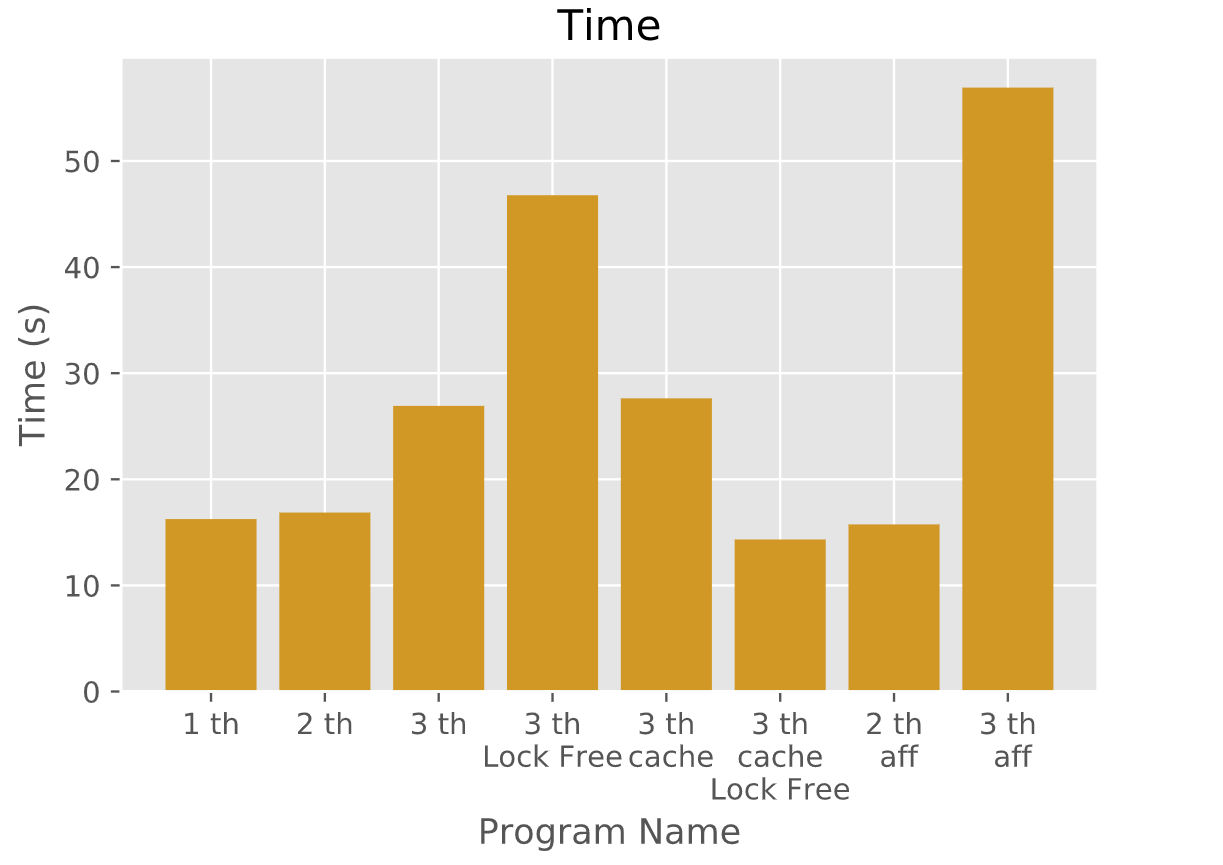
\includegraphics[width=.8\textwidth]{fig/lab-8}
  \caption{程序运行时间}
  \label{fig:RunningTime}
\end{figure}

\subsection{结果分析}

\paragraph{单线程} 通过性能分析工具,我们很容易就可以看出,
单线程版本的程序大部分的操作都是计算存储地址以及存储数据进入内存。
得益于程序自身对缓存的友好性以及现代CPU的乱序执行机制,
实际上内存访问并没有成为程序的瓶颈。

\paragraph{两线程} 双线程的情况和单线程没有太大的差别,
不过因为对于 apple 的操作和对于 orange 的操作可以同时进行,
运行时间减少了一点。

\paragraph{三线程 - 无锁} 在三线程时,因为 apple 的两个成员在缓存
的同一行内,对其进行多线程操作时的内存访问开始出现问题。我们知道
在 Intel CPU 内,各个核心的 L1 缓存以及 L2 缓存是独立的,L3 
缓存则是共享的。缓存的一致性由经过少许修改的 MESI 协议来确保。
因此在 apple 中的信息被任意一个核心修改后,其余核心的独立缓存内的这一行
都会失效,再次写入会直接写入进 L3,延时大大增加,这是造成运行
时间大幅增长的主要原因。同时,因为 LOAD 操作被之前未完成的 STORE 
操作阻挡造成的流水线阻塞也造成了一部分延时。

\paragraph{三线程 - 有锁}
此时的效果和串行地执行关于 apple.a 和 apple.b 的操作一样,延时增加大约一半。

\paragraph{三线程 - 无锁 - 缓存优化}
此时的运行时间和双线程类似。
此时 a 和 b 不在一个缓存行内,不同核心在修改这两个变量时候不用担心缓存的问题。

\paragraph{三线程 - 有锁 - 缓存优化}
无变化。

\paragraph{双线程 - CPU 亲和性}
无变化。

\paragraph{三线程 - CPU 亲和性}
时间大幅增加,推测是因为强制设置了 CPU 亲和性导致
线程被绑定到了任务较重的核心上。
由此得知,在现代 Linux 上,因为调度算法的完善,
通过设置 CPU 亲和性来提高性能的方式变得不再可靠,
甚至会有副作用。

\section{实验中的问题及心得}

在较新的 Linux 发行版下做实验二以及实验四时,
因为实验指导书资料的严重滞后,我们走了不少弯路。
后来是通过搜索引擎以及 Linux 内核自带的文档
逐一解决了这些问题,并在实验报告中记录下了
影响实验的 Linux 内核源码变动。如果可以的话,
希望能够在明年开操作系统课之前将实验指导书
翻新一下,让其至少不严重落后于时代潮流,彰显出
与计算机学科评估 {\textcolor{red}{\LARGE{\textbf{A}}}} 类
高校相称的教学水平。


\end{document}